\label{fs-acker-tracker}

This section introduces a novel substream management framework called \tracker\ that is suitable for cyclic dataflows and achieves the lower bound of network overhead. We also demonstrate that it provides all lifespan event properties defined in the previous section.

A substream management system should inform all processes that a substream ends, so the amount of extra traffic cannot be lower than $O(K||\Pi||)$. To achieve this lower bound, one can apply an additional agent (process) that receives information about substreams from processes and sends back information about terminated substreams. 

In this case, the fact that substream terminates is propagated through this agent without broadcasting between processes, so the amount of extra traffic can be linear by the number of processes. Such propagation method is suitable for cyclic dataflows because there is no need to forward service traffic through the cycles. Therefore, we design a {\em tracking agent} that:

\begin{enumerate}
    \item Receives signals from data producers that a substream has terminated.
    \item Watches for in-flight elements and substreams.
    \item Notifies dataflow processes when the substream ends {\em for them}, i.e., when they stop receiving elements which satisfy some predicate.
\end{enumerate}

The general scheme of the \tracker\ mechanism is shown in Figure~\ref{tracker_scheme}. A special (possibly distributed) tracking agent receives signals from data sources, fetches information about in-flight elements, and then decides where to send {\em end-of-substream notifications} (NEOSS).

This substream notifications distribution can be more efficient in terms of network traffic but provides new challenges. Before diving into implementation details, we should answer the following questions regarding \tracker\ framework:

{\bf Q1 How to monitor in-flight elements?} To detect that a substream ends, the tracking agent should receive the corresponding signal from data producers and ensure no substream in-flight elements. 

{\bf Q2 How to ensure bound guarantees?} While there are no longer special elements in the stream that denotes the substream end, we need to design soft and firm substream bound conditions based on NEOSS from the shared agent. 

{\bf Q3 How to provide a consistent termination events order?} Unlike punctuations, \tracker\ notifications are completely async with dataflow elements because they go through another network channel. Hence, dataflow items and notifications are not ordered, making it hard to ensure that the notifications order is consistent.

{\bf Q4 What functional and performance properties does the \tracker\ have?} \tracker\ framework is designed to eliminate the limitations of punctuations framework. We should demonstrate that it is suitable for cyclic dataflows as well as can provide lower network overhead.

\begin{figure}[htbp]
  \centering
  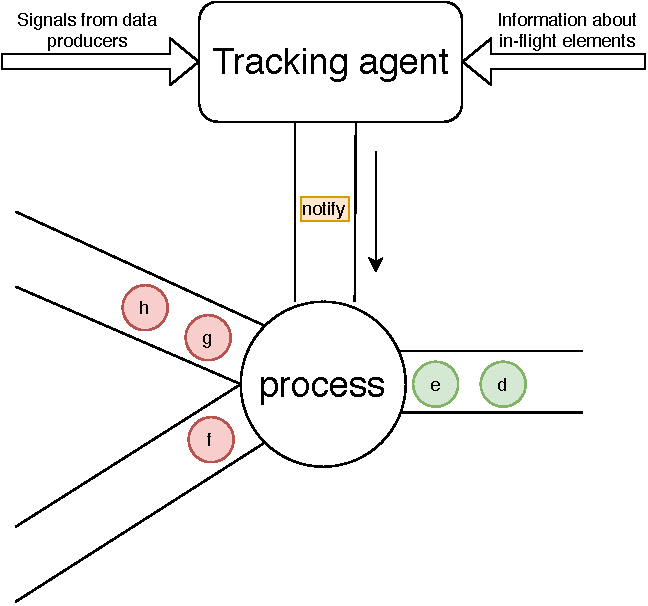
\includegraphics[width=0.20\textwidth]{pics/tracker-scheme.pdf}
  \caption{\tracker\ framework: tracking agent aggregates information about substreams and produces NEOSS}
  \label{tracker_scheme}
\end{figure}

\subsection{Answering Q1: How to monitor in-flight elements?}
To start tracking of a data element the system sends an $SND(pred, M, \emptyset)$ notification to the tracker. Then each process sends the following report messages on each $\langle proc, p, M, M' \rangle$ event:
\begin{enumerate}
    \item For all output elements $m \in M'$ for all substreams they belong to $pred(m) = 1$: $SND(pred, m, p)$
    \item For the input element $M$ and all satisfying substreams $pred(M) = 1$: $RCV(pred, M, p)$
\end{enumerate}
Further in this paper, we will denote them as {\em SND report} and {\em RCV report}. Note that this communication scheme is heavily optimized in practice. The order of $SND$ and $RCV$ messages is important because each pair of these events forms a chain ring, and sending $SND$ before $RCV$ links these rings together. We can use these chains to track data element processing for the whole workflow graph or its part.

Chains of $SND$ and $RCV$ messages allow the \tracker\ to track processing of a data element along with a workflow graph. This idea is not new and used in Apache Storm Acker but despite the technical similarity of the core idea\footnote{Good old XOR commutativity trick.}, Acker and \tracker\ play different roles in SPE. Acker ensures that the system entirely processed an input element and notifies the user when the processing runs out of time. \tracker\ tracks an entire substream and allows to define its bounds.

\subsection{Answering Q2: How to ensure bound guarantees?}
To detect a substream bound, a process needs to ensure that input channels will provide no more elements of this substream. In case of the punctuations framework, the watermark messages carry this guarantee. In case of shared agent, NEOSS messages play the same role. We can assume that each input channel $c$ comes from a segment of the workflow $W_c$ graph. NEOSS is sent to a process when:
\begin{itemize}
    \item for all incoming channels $c \in I_p$ corresponding segment $W_c$ contains no elements of the substream in-flight (has unpaired $SND$ report);
    \item all data providers have promised to send no more elements of the substream.
\end{itemize}
It is easy to show that we can join workflow segments for all incoming channels $W_p = \cup_{c\in I_p} W_c$ and track a single subgraph $W_p$ per process. Using the properties of NEOSS now we can define a soft bound criterion:
\begin{lemma}
Soft substream bound could be generated by following rule:
\begin{equation}
 \exists NEOSS \in B_p, \forall M\in B_p : \neg pred(M) \vee dst(M) \ne p
\end{equation}
\end{lemma}
\begin{proof}
If a substream data element is processed after the defined point in events order, it either comes from the mailbox or from one of the incoming channels $c \in I_p$. The first case contradicts $\forall m\in B_p : \neg pred(m)$. The second case could happen because a new substream element enters the system (source broke the promise) or a substream element inside the $W_p$ without the $SND$/$RCV$ chain (contradicts with $SND$/$RCV$ chains generation rule). 
\end{proof}

To satisfy the firm bound guarantee, one needs to hold elements that do not belong to the substream in the mailbox until NEOSS has arrived. This technique is quite similar to the punctuations alignment behavior mentioned in the previous section. If this condition is satisfied, then $\langle eoss_{firm}, Pred\rangle$ = $\langle eoss_{soft}, Pred\rangle$ for the \tracker.

\subsection{Answering Q3: How to provide the consistent termination events order?}
In the punctuations framework, such order is provided by design because punctuations and ordinary data items go through the same FIFO network channels. In \tracker\, this order should be enforced. Assume that SPE assigns to the messages a special totally ordered label $t(M)$. All messages generated by single processing inherit the label from the input message. 

In this case, if the order on $t(M)$ coincides with the order of input elements, then \tracker\ can produce the NEOSS events according to this order as well. In other words, \tracker\ can reorder the NEOSS events such that they will be consistent with the substreams order. An example of this concept is shown in Figure~\ref{tracker_ordering}. The substream containing element with $t=1$ ends before the substream containing element with $t=2$. As we can see, the order of NEOSS elements from \tracker\ coincides with $t(M)$.

\begin{figure}[htbp]
  \centering
  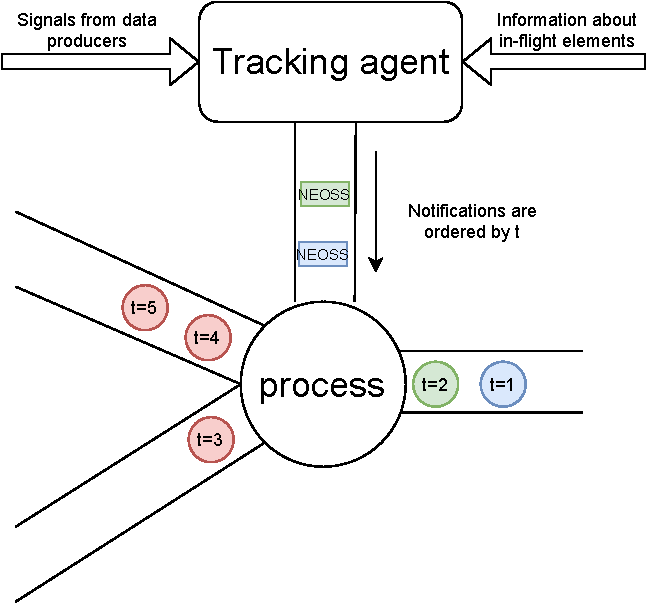
\includegraphics[width=0.20\textwidth]{pics/tracker-ordering.pdf}
  \caption{\tracker\ framework: tracking agent sends NEOSS elements according to the order on t(m)}
  \label{tracker_ordering}
\end{figure}

A vital question here is how to implement the assignment of ordered labels $t(m)$. One way is to use the {\em time oracle} service~\cite{10.14778/3055330.3055335} which can provide totally ordered labels. A simple alternative is discussed in the next section. 

\subsection{Answering Q4: What are the functional and performance properties of \tracker?}

\tracker\ does not require regular broadcasting of the elements to all computational nodes because all service traffic goes through a single agent. This change allows \tracker\ to have the following features by design:

\begin{enumerate}
    \item {\bf Cyclic dataflows support.} Because the tracking agent is monitoring the properties of in-flight elements without directly injecting service items into a dataflow, \tracker\ does not have the problem of throwing them through a cycle.
    \item {\bf Low network overhead.} Processes can send reports once per a fixed time period, so there is a constant time of such reports per a finite substream. The reports require $O(|\Pi|)$ extra messages, while the NEOSS events $O(K|\Pi|)$. The total amount is $O(K|\Pi| + |\Pi|) = O(K|\Pi|)$ that is optimal for the substream management problem. 
    \item {\bf Low latency and impact on SPE throughput.} Punctuations can be stuck by other data elements if they are sent with some delay after the last substream element. In \tracker, service traffic goes through other network channels that can reduce latency between actual substream termination and the corresponding event. Together with the low amount of service traffic, this scheme does not significantly reduce the throughput of an SPE, as we show in Section~\ref{fs-experiments}.
\end{enumerate}

At the same time, \tracker\ can provide both soft and firm bound guarantees along with the consistent order of notifications. A limitation of the \tracker\ framework is a potentially more complex implementation. The details of the straightforward implementation of the \tracker\ framework are discussed in the next section.